\section{Boundary conditions}\label{sec:lbm:bound}
In all physical situations, when solving a differential equations on a
domain, conditions for what is happening on the boundary of the domain
must be specified. So far, only the update rule for $\fii$ on the
interior of this domain have been treated. In this section we will
also define rules for the boundaries of the domain. The nodes in the
interior and the boundary will be referred to as \emph{interior nodes}
and \emph{boundary nodes} respectively. Typically, a boundary
condition in a macroscopic variable, e.g. velocity, is specified from
the physical problem. This condition must be translated into a
condition for the distribution function, $\fii$, on the statistical
level. In this section some, to this work, useful boundary conditions
will be formulated and discussed.

\begin{figure}
\begin{center}
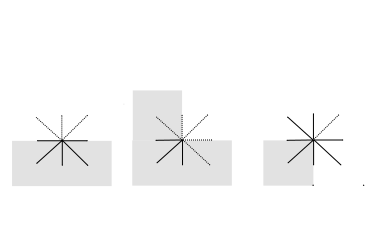
\includegraphics[width=0.9\textwidth]{fig/bb.pdf}
\end{center}
\caption{Three distinct boundary situations that in general has to be
  treated differently. From left to right, a straight boundary, a
  corner and an edge. Grey areas are outer of the domain. The Solid
  arrows corresponds to known directions of the distribution function
  and dotted lines to unknown.}
\label{fig:lbm:bounds}
\end{figure}

\subsection{Bounce-back boundaries}\label{sec:lbm:bb}
accuracy, e.g. second order accurate if placed between node planes...

\subsection{Slip boundaries}\label{sec:lbm:mirror}

\subsubsection{With momentum addition}\label{sec:lbm:mod_mirror}

\subsection{he-zou, constant density/velocity}\label{sec:lbm:hezou}

\subsection{Maybe something on non-local boundary conditions}
